\documentclass[10pt,a4paper]{article}
\usepackage[latin1]{inputenc}
\usepackage{amsmath}
\usepackage{amsfonts}
\usepackage{amssymb}
\usepackage{makeidx}
\usepackage{graphicx}
\usepackage[ruled,vlined]{algorithm2e}
\author{Artem Los}
\title{Hello}

\usepackage{marginnote}
\usepackage{verbatim} % for the box
\usepackage{fancyvrb} % for the box

\usepackage{listings}

\lstset{
% vilket spr�k vi anv�nder i v�ra kodlistings, s� att listings-paketet vet hur den ska highligta saker
language=Java,
% huruvida vi ska ha syntax highlighting
fancyvrb=true,
% hur stora tabstopp vi ska ha
tabsize=4,
% huruvida vi ska till�ta andra tecken �n a-z
extendedchars=\true
% hur breda listings vi vill ha (skriv exempelvis linewidth=0.5\textwidth f�r att f� listings som bara tar upp halva bredden av sidan)
linewidth=\textwidth,
% huruvida vi ska visa mellanslag
showstringspaces=false,
% huruvida vi ska bryta rader som �r f�r l�nga
breaklines=true,
% huruvida den ska f� bryta rader mitt i ord eller inte (true h�r betyder att den bara bryter mellan ord)
breakatwhitespace=true,
% indentera radbrytningar automatiskt
breakautoindent=true,
% l�gg in radnummer p� v�nster sida
numbers=left,
% hur stora radnumren ska vara
numberstyle=\tiny,
% hur l�ngt det ska vara mellan radnumren och koden
numbersep=8pt
}

\usepackage{pgf}
\usepackage{pgfpages}

\usepackage{fullpage}  % might require you to compile the page several times.



\begin{document}
\section*{Exercise 8.12}
\subsection*{a)}
We have the following class hierarchy:

\textbf{Person}
\begin{itemize}
	\item Teacher
	\item Student
	\subitem PhDStudent
\end{itemize}

\begin{enumerate}
	\item \verb|Person p1 = new Student();| is valid as Student is also a Person.
	\item \verb|Person p2 = new PhDStudent();| is valid as PhDStudent inherits from Student, which inherits from Person.
	\item \verb|PhDStudent phd1 = new Student();| is \textit{not} valid because a Student does not inherit from PhDStudent; that is, a student is not automatically a PhDStudent from the given class hierarchy.
	\item \verb|Teacher t1 = new Person();| is not valid, as Teacher is a subclass of Person. A Person can also be a Student, i.e. not a Teacher, which is why this declaration is illegal.
	\item \verb|Student s1 = new PhDStudent();| is perfectly fine since PhDStudent inherits the Student class.
\end{enumerate}

\subsection*{b)}

\begin{enumerate}
	\item \verb|s1 = p1;| is invalid as the Person class does not inherit from Student.
	\item \verb|s1 = p2;| is invalid by the same reasoning as above. \textit{p2} is a Person object and as we are trying to assign a Student object a Person object, it will not work.
	\item \verb|p1 = s1;| is valid because a Student inherits from a Person. This will, in other words, work!
	\item \verb|t1 = s1;| is not valid because there is no explicit connection between a Teacher object and a Student object apart from the fact that they inherit from the same class, that is, Person.
	\item \verb|s1 = phd1;| is valid because PhDStudent inherits from a Student.
	\item \verb|phd1 = s1;| is invalid because Student does not inherit from a PhD Student.
\end{enumerate}

\section*{Exercise 8.14}
Nothing has to be changed in the NewsFeed class when another subclass of Post is added because as long as a class inherits from Post, the current code will work. Right now, the addPost method does not explicitly specify the type of Post needed. It accepts all Posts, and thus subclasses of Post class.

\section*{Exercise 8.15}
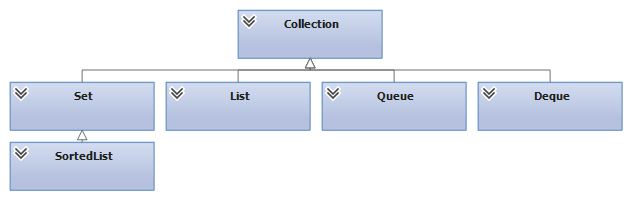
\includegraphics{dep.png}

\section*{Exercise 8.16}
\subsection*{LabClass}
\lstinputlisting{source/LabClass.java}
\subsection*{Person}
\lstinputlisting{source/Person.java}
\subsection*{Student}
\lstinputlisting{source/Student.java}
\subsection*{Instructor}
\lstinputlisting{source/Instructor.java}

\section*{Exercise 'exponentiation'}

\subsection*{Iterative}
The iterative exponentiation algorithm is equivalent to the function $\alpha$.

\begin{equation*}
\alpha(x,n) = \left\{
\begin{array}{lr}
x \times \alpha(x, n-1) & : n \ge 1\\
1 & : n = 0
\end{array}
\right.
\end{equation*} 

\textbf{Proof}
We want to show that this function is equivalent to taking a number $x\in \mathbb{R}$ to the power of a number $n\in \mathbb{N}$. Let $P_n$ denote the case when the exponent is $n$.
\\
\\
\textbf{Basis}
Let's take the case $n=0$.
\begin{eqnarray*}
\text{LHS} = \alpha(n, 0) = 1\\
\text{RHS} = n^0 = 1\\
\because \text{LHS} = \text{RHS}\\
\therefore P_0 = \text{true}
\end{eqnarray*}
\\
\textbf{Induction}
We assume that $P_n$ is true, i.e.
$\alpha(x,n) = x^n, \quad \forall n \forall x$ (*)\\
Then, for $P_{n+1}$:
\begin{equation*}
\alpha(x,n+1) = x \times \alpha(x,n) = x \times x^n = \text{using (*)} = x^{n+1}
\end{equation*}
$\therefore$ Since $P_0$ was shown to be true and assuming that $P_n$ is true, it was shown that $P_{n+1}$ is true also. Thus, by the principles of mathematical induction, $P_n$ is true for all $n\in \mathbb{N}$. $\square$
\\

\textbf{Time complexity} The time to execute this function is given by
\begin{equation*}
T(n) = \left\{
\begin{array}{lr}
T(n-1) + 1 & : n \ge 1\\
1 & : n = 0
\end{array}
\right.
\end{equation*} 
Sure enough, the closed form of $T(n)$ is:
\begin{equation}
T(n)=n+1 = O(n)
\end{equation}

\subsection*{Recursive}
The recursive implementation is a bit tricker. In order to prove that the algorithm represents exponentiation, we need to split it into two. The first part, i.e. $\forall n \le 4$, we know is true because we have shown that the iterative algorithm is true. It need not to be proved. The latter has to be proved, as it is not as clear what is going on. We do know that the last operation (where the recursive call is being made) is true because $\lfloor \frac{n}{2} \rfloor + \lfloor \frac{n+1}{2} \rfloor = n$, so the exponent is not altered. In other words, the recursive function will keep breaking up the exponent (without changing the value) until the exponent is less than or equal to $4$, when the iterative algorithm is called.

The time complexity for the recursive algorithm is given by (not including the iterative method call):
\begin{equation*}
T(n) = \left\{
\begin{array}{lr}
2T(n/2) + 1 & : n \ge 1\\
1 & : n = 0
\end{array}
\right.
\end{equation*} 
That is because it keeps breaking up the problem into two. The reason why the time complexity of all method calls to the iterative procedure were omitted is because they contribute with a constant number of operations. Given $n \implies T(n) = n+1$. Thus, $O(n)$, as we already have shown.
Using Master Theorem, since $0 < \log_22=1$, the time complexity of the recursive algorithm is also $O(n)$.

\end{document}

